%% LyX 2.0.0 created this file.  For more info, see http://www.lyx.org/.
%% Do not edit unless you really know what you are doing.
\documentclass[12pt,english]{article}
\usepackage{mathptmx}
\usepackage[T1]{fontenc}
\usepackage[latin9]{inputenc}
\usepackage{geometry}
\geometry{verbose,tmargin=1in,bmargin=1in,lmargin=1in,rmargin=1in}
\usepackage{babel}
\usepackage{graphicx}
\usepackage[unicode=true,pdfusetitle,
 bookmarks=true,bookmarksnumbered=false,bookmarksopen=false,
 breaklinks=false,pdfborder={0 0 0},backref=false,colorlinks=false]
 {hyperref}
\usepackage{breakurl}

\makeatletter

%%%%%%%%%%%%%%%%%%%%%%%%%%%%%% LyX specific LaTeX commands.
%% Because html converters don't know tabularnewline
\providecommand{\tabularnewline}{\\}

%%%%%%%%%%%%%%%%%%%%%%%%%%%%%% User specified LaTeX commands.
\date{}

\makeatother

\begin{document}

\title{Problem Set 3 Solutions}

\maketitle
Directions: Answer all questions. Clearly label all answers. Show
all of your code. Turn in the following to me via your dropbox (in
a folder labeled 'MatlabPS1.3') in Sakai by 11:59 p.m. on Thursday,
July 19, 2012: 
\begin{itemize}
\item m-file(s)
\item a log file (from off the cluster)
\item matsub.oXXXXX file
\item pdf version of your writeup with its \LaTeX source code
\end{itemize}
Put the names of all group members at the top of your writeup (each
student must turn in his/her own materials).
\begin{enumerate}
\item Practice with Matlab's graphics using \texttt{nhanes2d.mat} (from
PS2) --- visualizing descriptive evidence

\begin{enumerate}
\item See Figure 1. The data look quite normal.
\item See Figure 2. Once we look at the histogram, the data don't look nearly
as normally distributed as with the smoothed graph.
\item See Figure 3. Males clearly stochastically dominate females, meaning
that, at any point in their respective distributions, a male has more
red blood cells (as a percentage of blood volume) than a female.
\item See Figure 4. There is no such pattern by region.
\item See Figure 5. Whites/other stochastically dominate blacks in terms
of hematocrit percentage.
\end{enumerate}
\item Viewing model fit graphically

\begin{enumerate}
\item Graphing a predicted OLS plane

\begin{enumerate}
\item See Figure 6.
\end{enumerate}
\item Graphing actual data vs predicted OLS plane

\begin{enumerate}
\item See Figure 7. The model fit is not good at all. Even after conditioning
on 14 covariates and an intercept, there is still a large amount of
variation in hematocrit percentage that is unexplained.
\end{enumerate}
\end{enumerate}
\item Maximum likelihood estimation for a discrete dependent variable (high
blood pressure)

\begin{enumerate}
\item Logit estimates are found in Table 1.
\item Probit estimates are found in Table 2.
\item Table 3 compares the two sets of estimates. Some coefficients are
much closer than others, but they are still quite different overall.
Intepreting the model, high blood pressure is associated with being
older, black, having higher hematocrit, having a larger household
and being taller and heavier. Obviously, there isn't a model establishing
causality for any of these, so all we can say in terms of interpretation
is that the observed effects are associated with high blood pressure.
I was also surprised that having a heart attack was negatively related
to high blood pressure. This is probably due to heart attack victims
paying closer attention to their biometric data after suffering a
heart attack.
\item See Table 4 for a summary of the model fit. The logit fits better
in terms of $\overline{P}$, but the probit has a higher log likelihood
value.
\end{enumerate}
\end{enumerate}
\pagebreak{}

\begin{figure}
\caption{Kernel Density Plot of Hematocrit Percentage}


\bigskip{}


\centering{}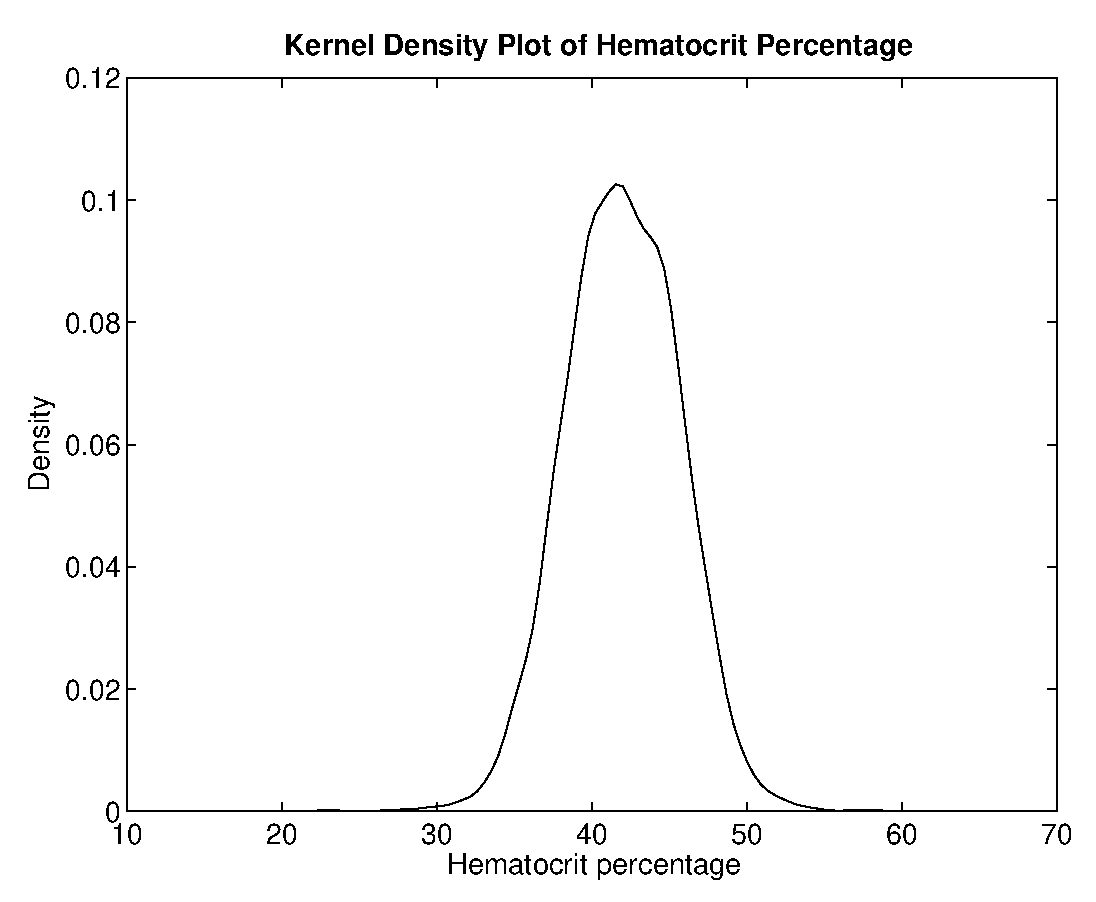
\includegraphics[scale=0.4]{fig1a}
\end{figure}


\begin{figure}
\caption{Distribution of Hematocrit Percentage}


\bigskip{}


\centering{}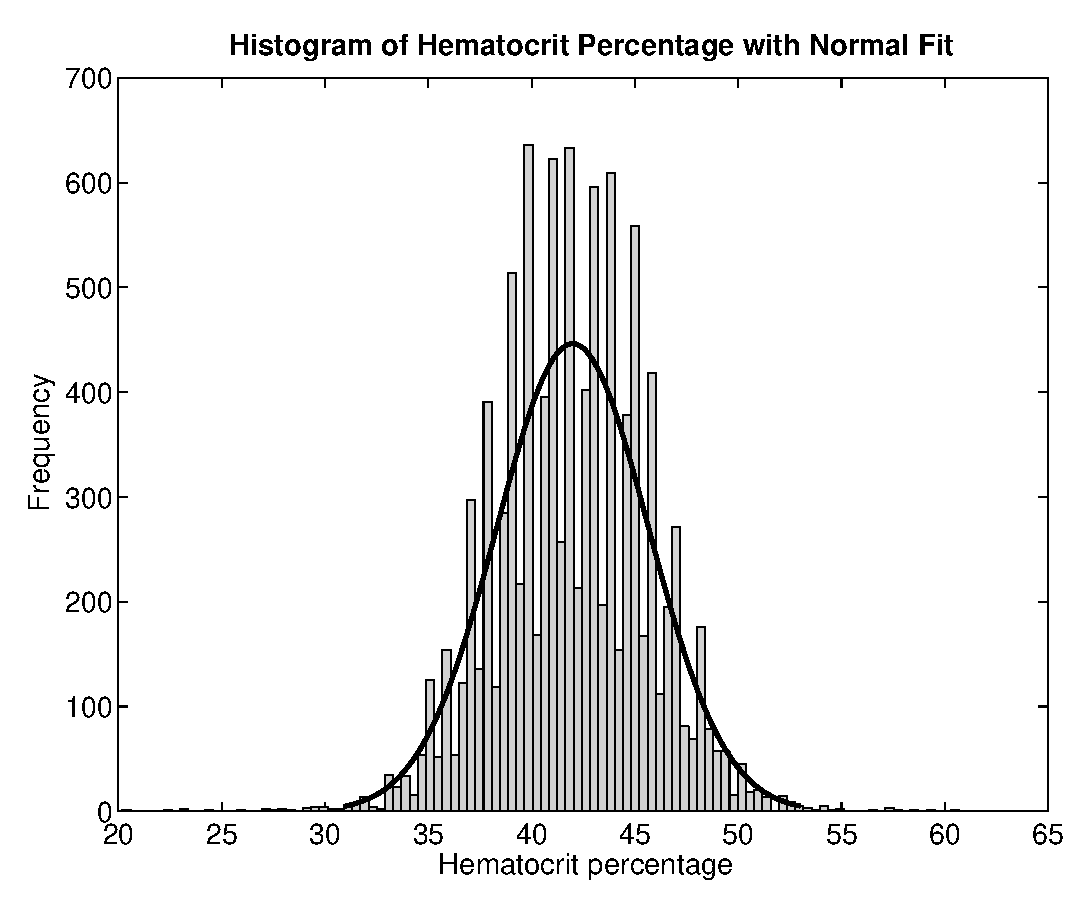
\includegraphics[scale=0.4]{fig1b}
\end{figure}


\begin{figure}
\caption{Empirical CDF of Hematocrit Percentage by Gender}


\bigskip{}


\centering{}\includegraphics[scale=0.4]{fig1c}
\end{figure}


\begin{figure}
\caption{Empirical CDF of Hematocrit Percentage by Census Region}


\bigskip{}


\centering{}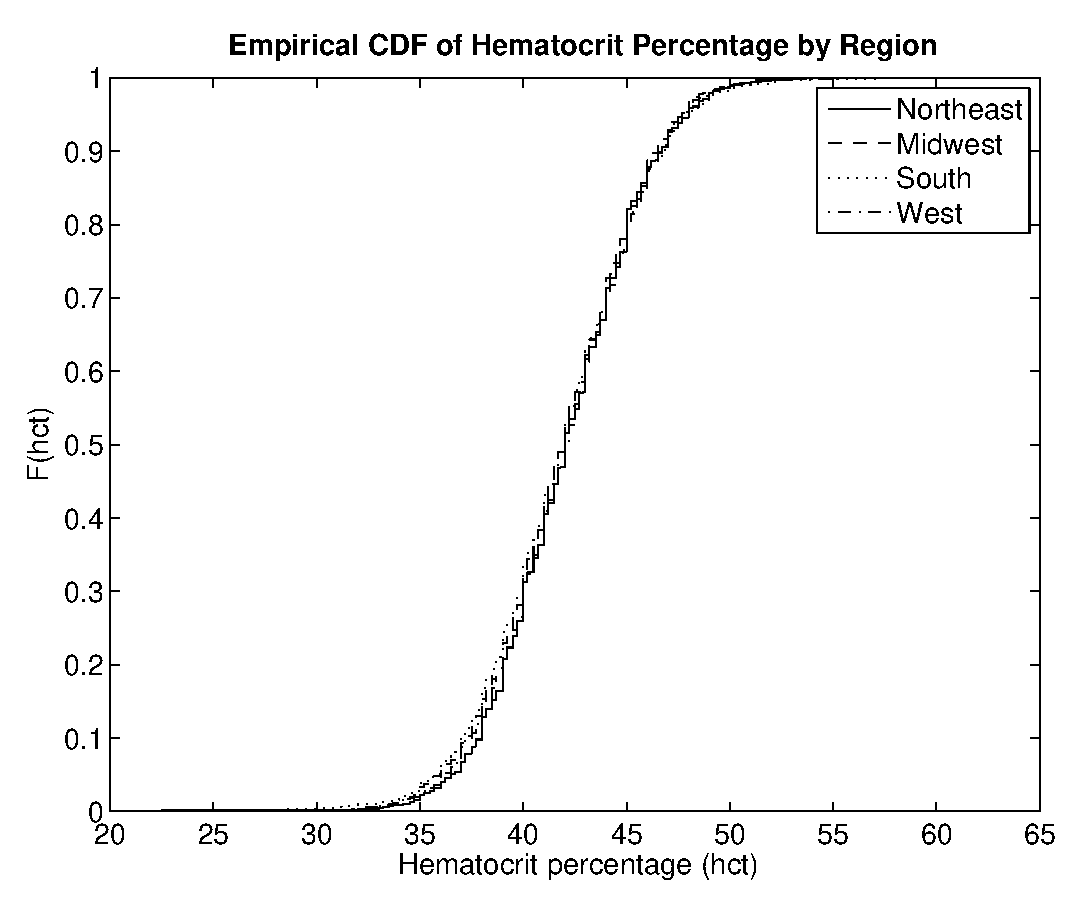
\includegraphics[scale=0.4]{fig1d}
\end{figure}


\begin{figure}
\caption{Empirical CDF of Hematocrit Percentage by Race}


\bigskip{}


\centering{}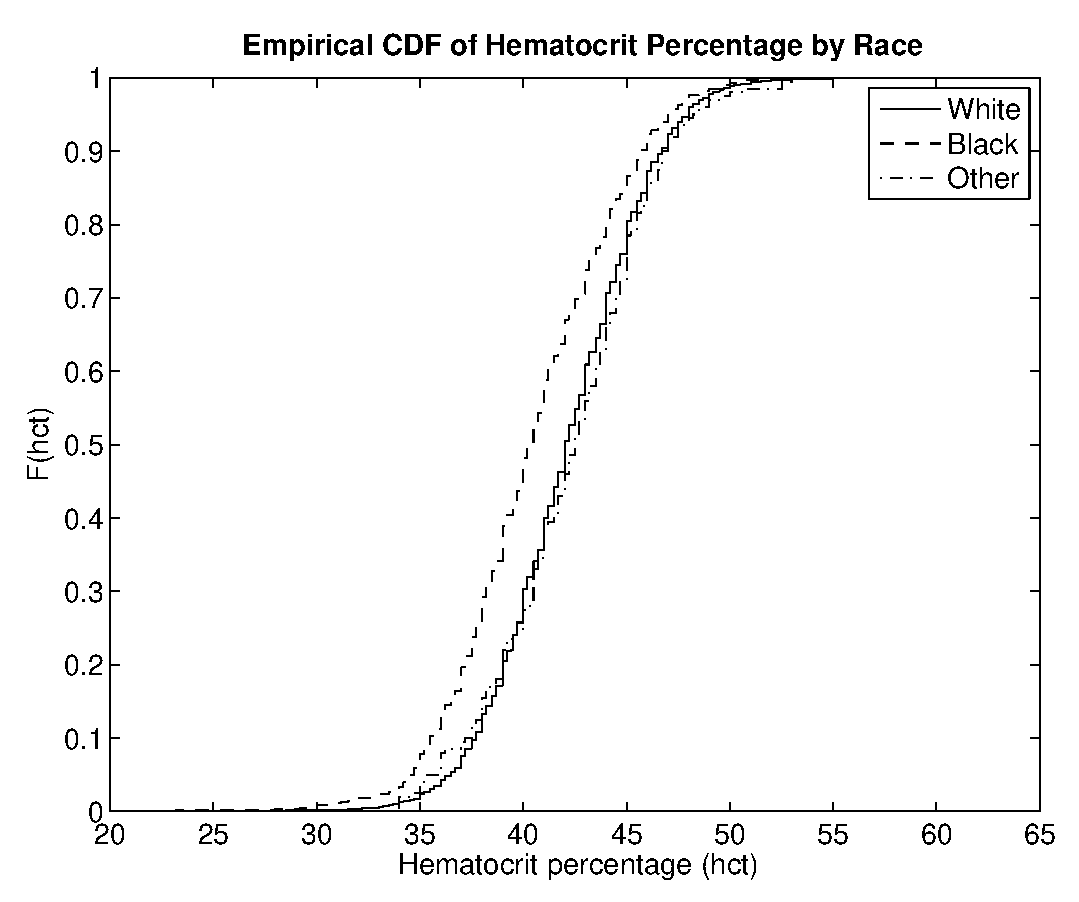
\includegraphics[scale=0.4]{fig1e}
\end{figure}


\begin{figure}
\caption{OLS plane predicting hematocrit percentage by height and weight}


\bigskip{}


\centering{}\includegraphics[scale=0.4]{fig2ai}
\end{figure}


\begin{figure}
\caption{OLS plane predicting hematocrit percentage by height and weight, with
actual data values}


\bigskip{}


\centering{}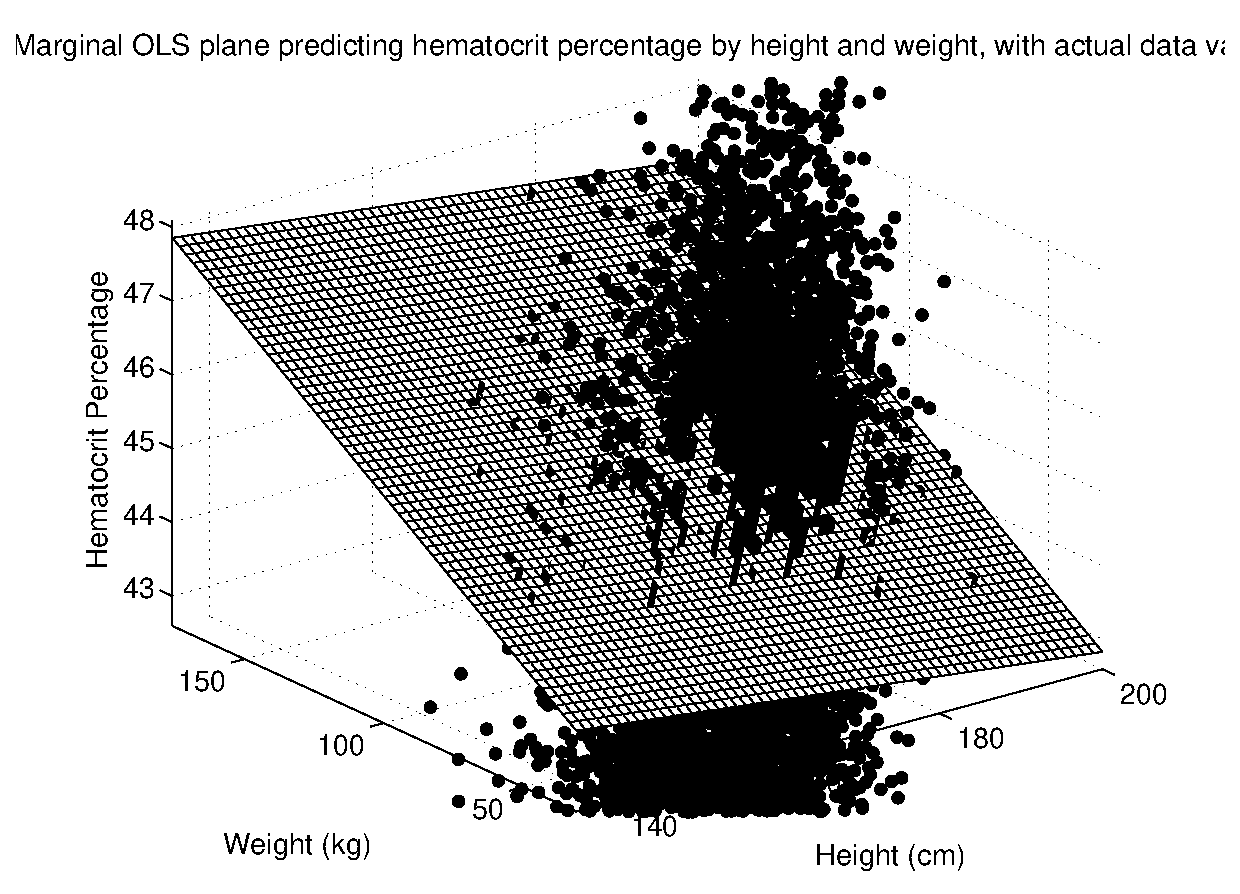
\includegraphics[scale=0.4]{fig2bi}
\end{figure}


\begin{table}
\begin{centering}
\caption{Logit MLE Estimates}

\par\end{centering}

\centering{}\bigskip{}
\begin{tabular}{ccc}
\hline 
Variable & $\hat{\beta}$ & Std Err.\tabularnewline
\hline 
Constant & -4.825 & 1.017\tabularnewline
age & 0.047 & 0.003\tabularnewline
black & 0.536 & 0.104\tabularnewline
other & 0.338 & 0.249\tabularnewline
heartatk & -0.266 & 0.132\tabularnewline
female & -0.091 & 0.099\tabularnewline
hematocrit \% & 0.031 & 0.010\tabularnewline
NE & 0.145 & 0.095\tabularnewline
MW & 0.039 & 0.090\tabularnewline
S & 0.106 & 0.090\tabularnewline
non central city & 0.124 & 0.091\tabularnewline
rural & 0.127 & 0.084\tabularnewline
height & -0.029 & 0.005\tabularnewline
weight & 0.048 & 0.002\tabularnewline
household size & 0.049 & 0.021\tabularnewline
\hline 
log likelihood & \multicolumn{2}{c}{-3,414.90}\tabularnewline
iterations & \multicolumn{2}{c}{169}\tabularnewline
$N$ & \multicolumn{2}{c}{10,349}\tabularnewline
\hline 
\end{tabular}
\end{table}


\begin{table}
\begin{centering}
\caption{Probit MLE Estimates}

\par\end{centering}

\centering{}\bigskip{}
\begin{tabular}{ccc}
\hline 
Variable & $\hat{\beta}$ & Std Err.\tabularnewline
\hline 
Constant & -2.539 & 0.552\tabularnewline
age & 0.025 & 0.001\tabularnewline
black & 0.307 & 0.057\tabularnewline
other & 0.189 & 0.133\tabularnewline
heartatk & -0.150 & 0.074\tabularnewline
female & -0.056 & 0.054\tabularnewline
hematocrit \% & 0.017 & 0.006\tabularnewline
NE & 0.074 & 0.052\tabularnewline
MW & 0.014 & 0.049\tabularnewline
S & 0.047 & 0.049\tabularnewline
non central city & 0.068 & 0.050\tabularnewline
rural & 0.080 & 0.046\tabularnewline
height & -0.016 & 0.003\tabularnewline
weight & 0.027 & 0.001\tabularnewline
household size & 0.023 & 0.011\tabularnewline
\hline 
log likelihood & \multicolumn{2}{c}{-3,401.55}\tabularnewline
iterations & \multicolumn{2}{c}{7,757}\tabularnewline
$N$ & \multicolumn{2}{c}{10,349}\tabularnewline
\hline 
\end{tabular}
\end{table}


\begin{table}
\begin{centering}
\caption{Logit vs. Probit}

\par\end{centering}

\centering{}\bigskip{}
\begin{tabular}{ccc}
\hline 
Variable & $\hat{\beta}_{logit}/1.6$ & $\hat{\beta}_{probit}$\tabularnewline
\hline 
Constant & -3.016 & -2.539\tabularnewline
age & 0.029 & 0.025\tabularnewline
black & 0.335 & 0.307\tabularnewline
other & 0.211 & 0.189\tabularnewline
heartatk & -0.166 & -0.150\tabularnewline
female & -0.057 & -0.056\tabularnewline
hematocrit \% & 0.020 & 0.017\tabularnewline
NE & 0.090 & 0.074\tabularnewline
MW & 0.024 & 0.014\tabularnewline
S & 0.066 & 0.047\tabularnewline
non central city & 0.077 & 0.068\tabularnewline
rural & 0.079 & 0.080\tabularnewline
height & -0.018 & -0.016\tabularnewline
weight & 0.030 & 0.027\tabularnewline
household size & 0.031 & 0.023\tabularnewline
\hline 
\end{tabular}
\end{table}


\begin{table}
\caption{Model Fit}


\bigskip{}


\centering{}%
\begin{tabular}{ccc}
\hline 
 & $\overline{P}$ & log likelihood\tabularnewline
\hline 
Data & .1290 & ---\tabularnewline
Logit Model & .1290 & -3,414.90\tabularnewline
Probit Model & .1287 & -3,401.55\tabularnewline
\hline 
\end{tabular}
\end{table}

\end{document}
